\documentclass{matmex-diploma-custom}

\begin{document}
% Год, город, название университета и факультета предопределены,
% но можно и поменять.
% Если англоязычная титульная страница не нужна, то ее можно просто удалить.
\filltitle{ru}{
    chair              = {Кафедра Системного Программирования},
    title              = {Скрытые Марковские модели переменного порядка для анализа
данных ChIP-seq},
    % Здесь указывается тип работы. Возможные значения:
    %   coursework - Курсовая работа
    %   diploma - Диплом специалиста
    %   master - Диплом магистра
    %   bachelor - Диплом бакалавра
    type               = {bachelor},
    position           = {студента},
    group              = 444,
    author             = {Атаманова Анна Михайловна},
    supervisorPosition = {},
    supervisor         = {},
    reviewerPosition   = {},
    reviewer           = {Лебедев С.\,А.},
    chairHeadPosition  = {д.\,ф.-м.\,н., профессор},
    chairHead          = {Терехов А.\,Н.},
%   university         = {Санкт-Петербургский Государственный Университет},
%   faculty            = {Математико-механический факультет},
%   city               = {Санкт-Петербург},
%   year               = {2015}
}
\filltitle{en}{
    chair              = {Chair of Software Engineering},
    title              = {Variable-length hidden Markov models for ChIP-seq data analysis},
    author             = {Anna Atamanova},
    supervisorPosition = {},
    supervisor         = {},
    reviewerPosition   = {},
    reviewer           = {Sergei Lebedev},
    chairHeadPosition  = {professor},
    chairHead          = {Andrey Terekhov},
}
\maketitle
\tableofcontents
% У введения нет номера главы
\section*{Введение}

\subsection*{Предметная область}
ДНК (дезоксирибонуклеиновая кислота) --- длинная двухцепочечная молекула, являющаяся носителем
генетической информации в биологических организмах. В клетках эукариот ДНК
находится в упакованном состоянии. Упаковка ДНК реализована с участием
специальных белковых комплексов --- нуклеосом. Химические модификации субъединиц
нуклеосомы, гистонов, могут влиять на плотность упаковки ДНК. Увеличение
плотности ДНК влияет на доступность соответствующих участков ДНК для внутренней
машинерии клетки.

%% TODO: чуть больше информации о важности изучения химических модификаций
%% хвостов гистонов

Иммунопреципитация хроматина с последующим секвенированием (chromatin
immunoprecipitation sequencing, ChIP-seq) --- это биологический протокол,
позволяющий получить информацию о наличие или отсутствии некоторой химической
модификации гистонов вдоль генома \cite{Johnson2007}. Суть метода заключается в
использовании антитела для отбора фрагментов ДНК, cвязанных с гистонами,
имеющими изучаемую химическую модификацию с последующим секвенированием. В ходе
секвенирования случайные фрагменты ДНК, читаются секвенатором в объёме,
достаточном для того, чтобы с большой вероятностью каждый фрагмент был прочитан
несколько раз. Затем для каждого полученного прочтения ищется соответствующий
ему участок последовательности генома (рис.~\ref{fig:chip-seq}). Обычно
прочтения, которым может соответствовать более одного участка в геноме,
исключают из рассмотрения.

\begin{figure}[h]
  \centering

%\begin{Verbatim}[commandchars=\\\{\}]
          CAAAAGACAAATAGTGATGTCACCAATCGAGC
          --------------------------------
               GACA ATA     GTCA   AATG
              AGAC   TAGTG TGTC
               GACA   AGTG TGTCA   ATCG

          00001100001110000110000001000000
%\end{Verbatim}
  \caption{Схематическое изображение выравнивания прочтений секвенатора (под чертой)
    на известную последовательность генома (над чертой).}
  \label{fig:chip-seq}
\end{figure}

Результаты эксперимента представляют в виде вектора длины генома, в котором
стоит 1, если в соответствующей позиции генома начинается хотя бы одно прочтение
и 0 в обратном случае.

%% TODO: описать разбиение на бины и ввести обозначения.

\subsection*{Формулировка проблемы}
Протокол хроматин-иммунопреципитации (как и большинство биологических
протоколов) не исключает наличие в результатах эксперимента
ошибок. Недостаточная специфичность антитела, наличие ошибок секвенирования
и нестабильность положения гистонов на ДНК приводят к возникновению сигнала не
зависящего от наличия изучаемой модификации гистонов.
\\
По этому для дальнейшего анализа результатов эксперимента требуется построение некоторой вероятностой модели, способной отделять ошибки, а также выявлять зависимости и кратко описывать структуру данных.

\section{Постановка задачи}
Целью данной работы является:
\begin{enumerate}
\item
Изучение скрытых марковских моделей переменного порядка
\item
Реализация скрытой марковской модели переменного порядка
\item
Применение модели к результатам биологического эксперимента ChIP-seq 
\end{enumerate}

\section{Обзор существующих решений}
Большинство существующих моделей (TODO: ref) для данных
хроматин-иммунопреципитации основано на аппарате скрытых Марковских моделей
второго порядка с Пуассоновскими испусаниями. Использование распределения
Пуассона для покрытия, опирается на предположение о том, что в каждой
позиции генома в среднем начинается одинаковое количество прочтений. Марковский
процесс, как правило, имеет два состояния $+$ --- сигнал есть и $-$ --- сигнала
нет. Второй порядок модели означает, что состояние некоторого окна зависит только
от состояния его прямого предшественника.

Использование моделей второго порядка объясняется тем, что количество параметров
модели, а также сложность её обучения и использования экспоненциально зависят от
порядка, то есть, модель порядка $m$ требует оценки $2^m$ параметров.

%% TODO: четче объяснить привлекательность модели второго порядка и перейти к
%% цели работы.

В настоящее время, в качестве семейства искомых моделей, активное приминение находит HMM (Hidden Markov Model)\cite{Rabiner1989} второго порядка с Пуассоновским испусканием.
Данное семейство допускает предположение о том, что каждое состояние (наличие/отсутствие белка в заданной части генома) завист только от одного предыдущего.
Можно ограничиться и более лояльным допущением о том, что состояние зависит от $n$ предыдущих состояний, однако такое допущение резко увеличивает сложность модели ($O(2\textsuperscript{n})$ параметров). Также, сложность заключается в подборе этого $n$ и переобучении в случае, если не все состояния имеют одинаковые длины контекстов зависимости.

\section{Скрытые марковские модели переменного порядка}
\subsection{Марковские модели}
\textbf{Определение.} Последовательность случайных величин $ \{X_{i}\}_{i \in Z}$ называется \emph{цепью Маркова порядка $ m $}, если $ \forall t\in Z $

$ P(X_{t} = x
Последннее замечание подводит к идее использования VOHMM (Variable Order Hidden Markov Model)\cite{Wang2006}
_{t}|X_{t-1}=x_{t-1},X_{t-2}=x_{t-2} ... X_{-\infty}=x_{-\infty})$ = 
$ P(X_{t} = x_{t}|X_{t-1}=x_{t-1},X_{t-2}=x_{t-2} ... X_{t-m+1}=x_{t-m+1}) $ 
\\\\
\textbf{Определение.} Марковская цепь является \textit{однородной}, если вероятностное распределение переходов $P(X_{t} = x_{t}|X_{t-1}=x_{t-1},X_{t-2}=x_{t-2} ... X_{t-m+1}=x_{t-m+1})$ едино для всех $ t $.
\\\\
Далее будем обозначать просто $ P(x_{t}|x_{t-1}..x_{t-m+1})$
\\\\
\textbf{Определение.} \emph{Марковской моделью (Markov Model (MM)) порядка $ m $} называют вероятностную модель, описывающую однородный марковский процесс порядка $ m $.
Параметрами модели являются множество состояний $ S = \{1..n\} $ и множество переходов $ A = \{a(q; x^{m})\}_{q \in S, x^{m} \in S^{m}}$, где $a(q; x^{m}) = P(q|x^{m})$. 
\\\\
\subsection{Скрытые марковские модели}
\textbf{Определение.} \emph{Скрытая Марковская модель (Hidden Markov Model(HMM)) порядка $ m $} - вероятностная модель, параметрами которой являются множество скрытых состояний $ S = \{1..n\} $, множество переходов $ A = \{a(q, x^{m})\}_{q \in S, x^{m} \in S^{m}}$ и множество распределений испусканий $ B = \{b(y,x)\}_{y \in R^{l}, x \in S}$, где $ b(y, x) = P(y|x)$. 
\\
Такая модель описывает цепь $\{Y\}_{i \in Z}$, если ее состояния были испущены из состояний марковской цепи $\{X_{i}\}_{i \in Z}$ с параметрами $ A $ согласно распределению $ P(y|x) $, и $ P(y_{t}|y_{t-1}..y_{t-m+1}) = P(x_{t}|x_{t}..x_{t-m+1})P(y_t|x_t)$  
\\\\
На рисунке (Рис \ref{ris:image}) схематично представлена скрытая марковская модель порядка 2.
\\
\begin{figure}[hbtp]
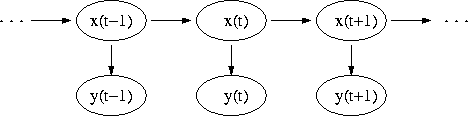
\includegraphics[scale=0.4]{img/Hmm_temporal_bayesian_net.png}
\centering
\caption{HMM order 2}
\label{ris:image}
\end{figure}
\\\\
\subsection{Скрытые Марковские модели переменного порядка}
\textbf{Определение.} \textit{Контекстное дерево} - дерево (бор), в котором каждая внутренняя вершина имеет $ n $ ребер соответствующих состояниям $ \{1..n\} $ и метку, которая является конкатенацией метки на ее родителе и метки ребра от него. Корень помечен пустой строкой. 
\\\\
\textbf{Определение.} \textit{Скрытая марковская модель переменного порядка (Variable-Length Hidden Markov Models (VLHMM))}- вероятностная модель, параметрами которой являются множество скрытых состояний $ S = \{1..n\} $, конечное множество контекстов $ C=\{c_{i}\}_{i} $, где $ c_{i} $ - листья некоторого контекстного дерева, множество переходов $ A = \{a(q; c)\}_{q \in S, c \in C}$ и множество распределений испусканий $ B = \{b(y,x)\}_{y \in R^{l}, x \in S}$, где $ b(y, x) = P(y|x)$.  
\\\\\\
\subsection{Обучение модели VLHMM}
{\large Задача:} 
\\
По цепи наблюдений $ Y = (y_{1}, ... y_{T}) $ найти модель VLHMM c параметрами $ \Lambda$, с минимальными по длине контекстами и максимальным правдоподобием. 
\footnote{Параметр алгоритма $ \epsilon $ определяет допустимое отклонение распределений}
\\
Другими словами, найти
\\
$\Lambda = \arg\!\min_{\Lambda}{\{|\Lambda(C)|\;|\Lambda \in \arg\!\max_{\Lambda}{\{P(Y|\Lambda)\}}\}}$
\\\\
{\large Алгоритм:}
\\
Параметры алгоритма: 
$ m $ - максимальная длина контекста, 
$ \epsilon_{EM} $ - барьер для остановки EM,
$ \epsilon_{prune} $ - барьер для обрезания дерева
\\
\begin{enumerate}
\item Инициализация контекстов.
\\
$ C_{0} = \{c| c\in S^{m}\}$
\\
Начальное распределение переходов произвольное.
\footnote{В определенных случаях (Gauss, Poisson) частотное распределение, полученное из цепи алгоритмом k-means (k=m), ускоряет работу}
\\
\item EM (Expectation–Maximization algorithm).
\\
Пересчет производится подобно алгоритму Baum-Welch для HMM
\\
\begin{enumerate}
\item Expectation
\\
Вводятся дополнительные параметры:
\\
$ \alpha_{t}(c) = P(y_{1}^{t}, c(x_{t})=c| \Lambda)$
\\
$ \beta_{t}(c) = P(y_{t+1}^{T}| c(x_{t})=c, \Lambda))$
\\
$ \gamma_{t}(c) = P(x_{t}=c|Y,\Lambda) $
\\
$ \xi_{t}(q;c) = P(c(x_{t})=c, x_{t+1} = q| Y, \Lambda)$
\\
с помощью которых итеративно пересчитываются параметры модели
\\
$ \alpha_{0}(c) = p(c)b(y_{0},c)$, 
$ \alpha_{t+1}(c) = \sum_{q \in S, c'=C(cq)}{\alpha_{t}(c')a(c[0];c')b(y_{t+1},c[0])}$
\\
$ \beta_{T}(c) = 1$, 
$ \beta_{t}(c) = \sum_{q \in S, c'=C(qc)}{a(q;c)b(y_{t+1}, c'[0])\beta_{t+1}(c')}$
\\
$p = P(Y|\Lambda) = \sum_{c \in C}\alpha_{T}(c)$
\\ 
$ \gamma_{t}(c) = \frac{\alpha_{t}(c)\beta_{t}(c)}{p}$
\\
$p(c) = \sum_{t}\gamma_{t}(c)$
\item Maximization
\\
$ \xi_{t}(q;c) = \frac{\alpha_{t}(c)a(q;c)b(y_{t+1},q)\beta_{t+1}(qc)}{p} $
\\
$ a(q; c) = \frac{\sum_{t}\xi_{t}(q,c)}{p(c)}$
\\
Пересчет $ B $ зависит от принятого семейства моделей испусканий и производится с помощью $ \gamma $ в точности также как и в алгоритме Baum-Welch.
\\
В случае распределения Пуассона
$b(.|c) ~ Poisson(\lambda_{c})$ 
\\
$ \lambda_{c} = \frac{\sum_{t}{\gamma_{t}(c)y_{t}}}{\sum_{t}{\gamma_{t}(c)}}$
\end{enumerate}
Пересчет EM проходит до тех пор пока разница правдоподобий между итерациями не будет меньше $ \epsilon_{EM}$
\\
\item Обрезание дерева.
\\
Если существует внутренний лист $ s $ такой, что $ \forall q \in S \; P(sq)kl(sq, s) < \epsilon_{prune} $ (дети не уточняют родителя), то $ s $ становитcя листом, а все его потомки обрезаются.
\\
$kl(u, w) = \sum_{q' \in S} P(q'|u) log\frac{P(q'|u)}{P(q'|w)}$ - расстояния Кульбака-Лейблера для апостериорных распределений.
\\
\item Если на третьем шаге ничего не произошло, то алгоритм заканчивет работу, 
иначе происходит обновление матрицы $ a $ для новых контекстов
\\
$ a(q; c) = P(q| c) $
\\
и алгоритм переходит на второй шаг.
\\
\end{enumerate}
Обозначения: 
\\
$ c[0] $ - состояние, являющееся началом контекста $ c $
\footnote{Контекст $ c $ представляем как последовательность состояний $c[0]c[1]...c[l-1]$, где $ l $ - длина контекста.}
\\
$ c(x_{t}) $ - контекст состояния $ x_{t} $ 
\\
$ C(s) $ - листья, являющиеся потомками $ s $, если $ s $ принадлежит дереву 
\\
$ C(s) $ - контекст максимальной длины, являющийся префиксом $ s $, если $ s $ не принадлежит дереву 
\\\\
\textbf{Замечание.}  Вероятностные переходы на листьях задают вероятностные переходы на всем дереве

$ p(q|s) = \frac{\sum_{c \in C(s)} {p(q|c)}}{\sum_q\sum_{c \in C(s)} {p(q|c)}} $ 
\\\\\
\textbf{Замечание.} При пересчете верятности могут очень близко подходить к нулю, что негативно сказывается на точность расчета. Для избежания этой проблемы все расчеты проходят не с вероятностями, а с логарифмами от них.
\\\\\
\textbf{Замечание.} EM может застревать в локальных максимумах функции правдоподобия.
\\\\\
\subsection{Обучение на нескольких выборках}
Пусть дано $ N $ выборок $ \{Y^{1} ... Y^{N}\}$
\\
EM
\begin{enumerate}
\item Expectation
\\
Считаем для каждой выборки  $\alpha^{d}, \beta^{d}, \gamma^{d}, \xi^{d}$
\\
Общая $\gamma$ - конкатенация гамм на выборках
$ \gamma = [\gamma^{1}, .... ,\gamma^{N}] $
\\
$ p = \prod_{d}{p^{d}}$
\item Maximization
\\
$ a(q;c) = \frac{\sum_{d}{\sum_{t}{\xi^{d}_{t}(q;c)}}}{\sum_{t}{\gamma_{t}(c)}} $
\\
и нормировка
$ a(q;c) = \frac{a(q;c)}{\sum_{q}{a(q;c)}} $
\\
Параметры испускания считаются по общей $ \gamma $ так же, как в обычной моделе.
\end{enumerate}

\section{Simulation}
План проверки работы VLHMM.
\begin{enumerate}

\item
Генерация параметров $ \Lambda $ начальной модели VLHMM.
\item
Сэмплирование выборки $ Y $ из заданной модели.
\item
Обучение новой модели на $ Y $. 
\\Получение предсказанных параметров $\hat{\Lambda}$.
\item
Сравнение параметров $ \Lambda $ и $ \hat{\Lambda} $.
\end{enumerate}

Ниже приведены два примера теста.
\begin{itemize}
\item Смесь.
\begin{enumerate}
\item Параметры начальной модели: $\Lambda = (C, A, B)$ 
\\множество контекстов $C = \{""\}$, множество переходов $A = \{[0.4, 0.6]\}$, множество распределений испусканий $B = \{Pois(2.61), Pois(15.34)\}$. 
\item Выборка длиной $ T = 1000 $
\item Обучение проходило начиная с полного дерева глубиной $ m  = 3$, рандомным распределением переходов. 
\\Остальные параметры алгоритма: барьер для обрезания $ \epsilon_{prune} = 0.01$, барьер для остановки EM $ \epsilon_{EM} =  0.15 $      
\item На рисунке \ref{ris:img_mixture_main} представлен график логарифма правдоподобия по всем итерациям, реальное и предсказанное деревья переходов.
\\Параметры предсказанной модели $\hat{\Lambda} = (\hat{C}, \hat{A}, \hat{B})$  
\\$\hat{C} = \{""\}, \hat{A} = \{[0.41, .59]\}, \hat{B} = \{Pois(2.7), Pois(15.3)\}$.
\\Параметры исходной и предсказанной модели схожи.
\begin{figure}[ht]\centering
	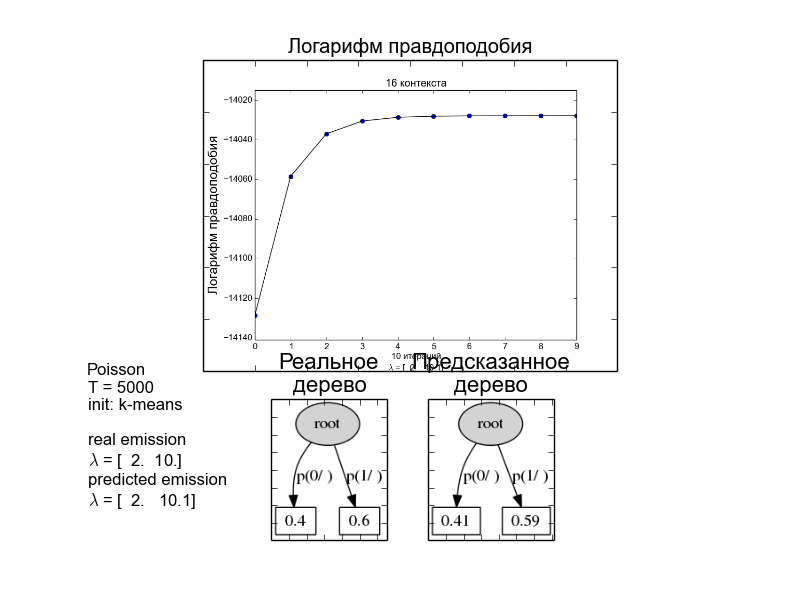
\includegraphics[scale=0.5]{img/sample_mixture/main.png}
	\centering
	\caption{Результат работы алгоритма VLHMM на смеси Пуассонов}
	\label{ris:img_mixture_main}
\end{figure}
\end{enumerate}
\item
Более интересный случай. 
\begin{enumerate}
\item Параметры начальной модели: 
\\множество контекстов и множество переходов представлены на рисунке \ref{ris:sample_real_trie}, распределения испусканий - $Pois(13.1), Pois(36.1)$. 
\item Выборка длиной $ T = 10000 $
\item Обучение начиналось с полного дерева глубиной $ m = 4 $, остальные параметры алгоритма те же, что и у примера выше.
\item Предсказанное алгоритмом дерево переходов и график логарифма прадоподобия представлены на рисунках \ref{ris:sample_predicted_trie},\ref{ris:sample_log_likelihood}
\\Распределения предсказанных испусканий - $Pois(13), Pois(35.9)$.
\begin{figure}[ht]\centering
	\parbox[b]{ 0.49 \textwidth}{
	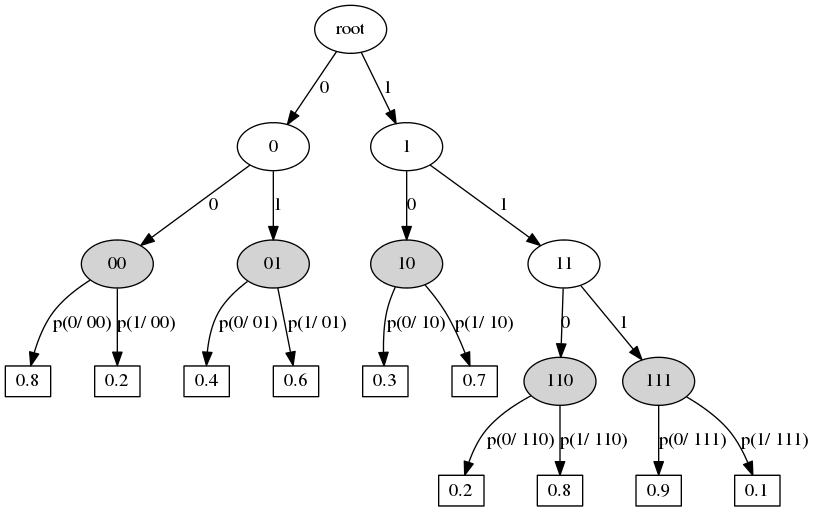
\includegraphics[scale=0.3]{img/sample/real_trie_.png}
	\centering
	\caption{ Реальное дерево }
	\label{ris:sample_real_trie}
	
	}
\hfil \hfil%раздвигаем боксы по горизонтали
\begin{minipage}[b]{0.49 \textwidth}
	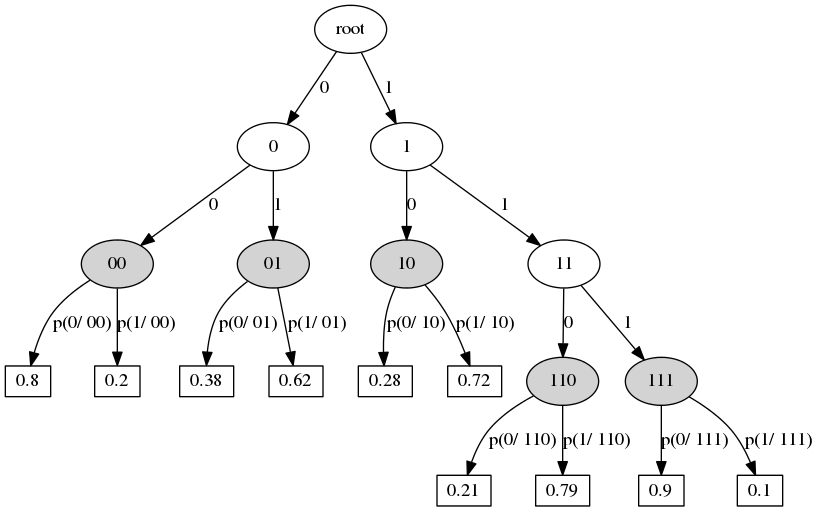
\includegraphics[scale=0.3]{img/sample/trie_.png}
	\centering
	\caption{ Предсказанное дерево }
	\label{ris:sample_predicted_trie}
\end{minipage}
\end{figure}
\begin{figure}[hbtp]
	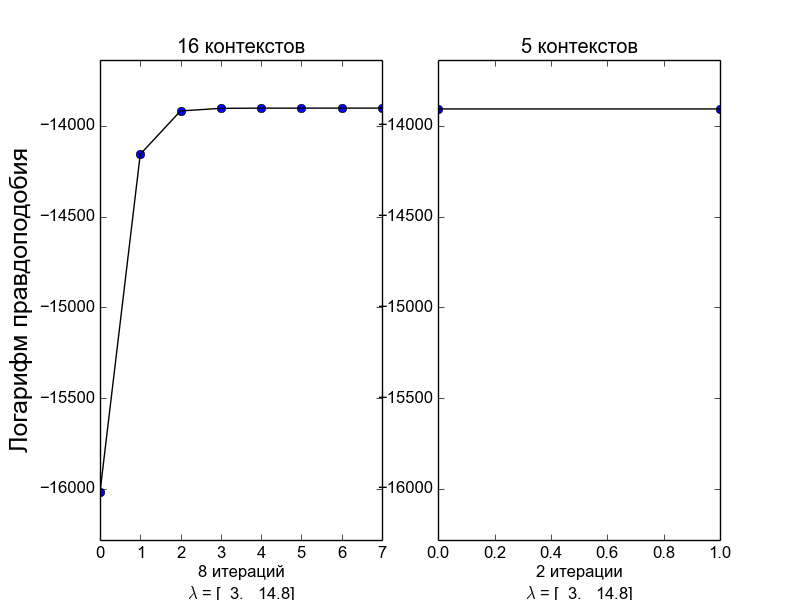
\includegraphics[scale=0.4]{img/sample/plot_.png}
	\centering
	\caption{ График роста логарифма правдоподобия }
\label{ris:sample_log_likelihood}
\end{figure}
\\
\end{enumerate}
\end{itemize}


\section{Chip-seq, реальные данные}


\section{Оценка модели}

\section*{Заключение}

\bibliographystyle{plain}
\bibliography{diploma.bib}
\end{document}
